\begin{figure}[tbp]
\centering
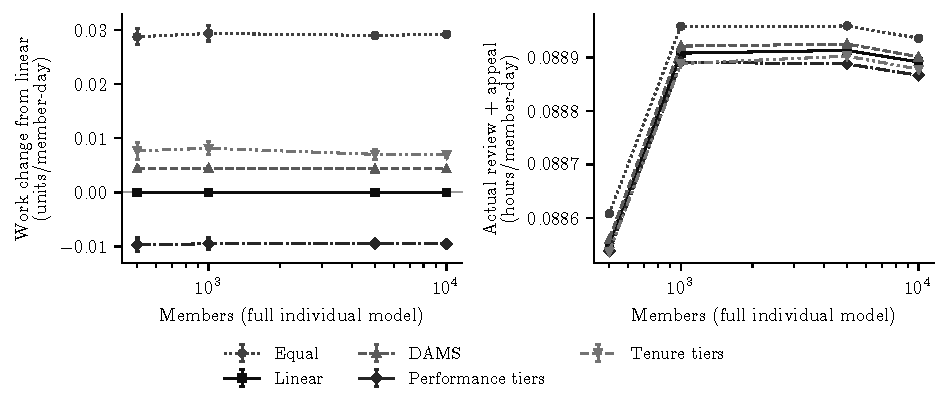
\includegraphics[width=\textwidth]{figures/results/organizational-scale.pdf}
\caption{Exploratory organizational scale comparisons: eight independent worlds at each of 500, 1,000, 5,000 and 10,000 full individual members, four guilds, two sites and 30 days. Left: paired work effect and descriptive 95\% Monte Carlo interval. Right: actual review and appeal service hours, excluding unused reservations and other unmodeled governance costs. Curves connect measured sizes, without extrapolating organizational benefits. Population growth also enlarges each fixed guild; guild count is not validator count.}
\label{fig:organizational-scale}
\end{figure}
\begin{figure}[tbp]
\centering
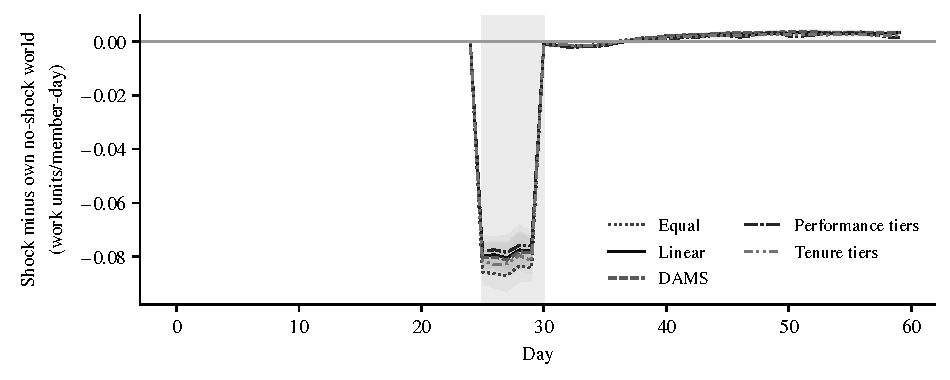
\includegraphics[width=\textwidth]{figures/results/shock-recovery.pdf}
\caption{Matched shock and no-shock output trajectories for five policies: eight independent world pairs per policy, 120 members and 60 days. Site 0 experiences a 0.7 output multiplier on days 25--29. Lines show paired mean work differences with pointwise descriptive 95\% Monte Carlo bands; zero is the matched no-shock outcome, not a pre-shock trend forecast. Repository recovery time is the first post-shock start of three days at least 99\% of own control output, with unrecovered worlds retained.}
\label{fig:shock-recovery}
\end{figure}
